\documentclass[a4paper, 11pt, oneside]{scrartcl}
\usepackage{lpp}
\usepackage{listings}
\usepackage{booktabs}
\usepackage{multirow}
\usepackage{mathpazo}
\usepackage{amsmath,amsfonts,amssymb,amsthm}
\usepackage{mathtools}
\usepackage{commath}
\usepackage{amsmath}
\usepackage{graphicx}
\usepackage{epstopdf}
\epstopdfsetup{outdir=./}
\usepackage[utf8]{inputenc}
\usepackage[english]{babel}
\usepackage[document]{ragged2e}



\begin{document}

\mtitle{Homework 8: The 2D Ritz-Galerkin  method for the Poisson-equation  }

\mauthor{Nelson Martin Sanchez Martinez}{}


\maff{Numerical Methods for Partial Differential Equations}{nelson.sanchez@rwth-aachen.de}{}

\mabstract{\ In this paper is discussed an implementation to solve a 2 dimensional Poisson equation problem with homogeneous boundary conditions using the Ritz-Galerkin method with 2 different meshes (triangle elements). The error is evaluated in the $L^2$ norm giving the following results for the structured mesh with 121 grid points and 200 triangles of 0.03355839110269951 and for the unstructured mesh with 81 grid points and 128 elements of 0.006475373360939617.


\section{The implementation}

\subsection{The Ritz-Galerkin method}

\ The problem for which this implementation was created has the following definition:
\begin{center}

\graphicspath{{C:/Users/toshiba/Documents/Sim_Sciences_1_Semester/1_Sem_Materias/NMPDE/HW7/tex-template/}}

    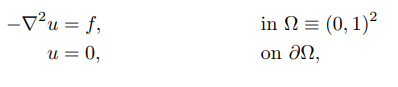
\includegraphics[width=8cm]{{C:/Users/toshiba/Documents/Sim_Sciences_1_Semester/1_Sem_Materias/NMPDE/HW8/tex-template/PRO-DEF.png}}
    
   \hfill
   
    \ Image 1: Set of conditions for this particular problem, at a first glance, rather simple.
\end{center}

\subsection{Setting the initial configuration}

As usual we define the functions that are needed for our solution to work.  As we know that we'd have to solve a system of equations of the shape $Ax = F$  ,from which we don't draw any conclusion regarding its conformation (of course, we know it's an invertible matrix, since the problem is well-posed for the Ritz-Galerkin approximation) therefore, in the eyes of generality, a built-in python routine has been chosen to solve this system. It's worth to notice that this implementation closely follows the guidelines given by tutorial 13 and 14 in the Professor Georg May's winter 2018 / 2019 lectures in Numerical Methods for Partial Differential Equations (May, 2019).

As promised, the following are the functions used in the implementation:
 \begin{center}
\begin{lstlisting}[language=Python, caption={Pyhton, Function definition },frame=single,breaklines=true]

## Name is suggestive enough
def mesh_selector(n):
    if n == 0:
        return  r"C:\Users\toshiba\Documents\Sim_Sciences_1_Semester\1_Sem_Materias\NMPDE\HW8\str10_test.csv"
    if n == 1:
        return r"C:\Users\toshiba\Documents\Sim_Sciences_1_Semester\1_Sem_Materias\NMPDE\HW8\unstr8_test.csv"
##As in the definition of the problem
def f(x,y):
    return  np.pi**2*np.sin(np.pi*x)*np.sin(np.pi*y)
    
##Exact solution of the problem
def fsol(x,y):
    return  np.sin(np.pi*x)*np.sin(np.pi*y)
##Evaluate matrix products
def matmat(m,n,mn,u,v):
    result = np.zeros((m,n))
    for i in range(0,m):
       for j in range(0,n):
           for k in range(0,mn):
               result[i][j] += u[i][k] * v[k][j]
    return result
##Personalized function to transpose arrays (2D)
def transpose(m,n,A):
    B = np.zeros((n,m))
    for j in range(m):
        for k in range(n):
            B[k][j] = A[j][k]
    return B
##Personalized determinant by chunks
def chunkdet(a,b,c,d):
    return np.abs((a*d) - (c*b))
    
       
\end{lstlisting}


Now we proceed to extract the information from the meshes. To do this somewhat easier, the given files were turned into a comma separated file and then extended with an additional column of zeros (to match the dimensionalities of the x and y coordinates with the connectivity of the triangles). The following implementation was created:


\begin{center}
\begin{lstlisting}[language=Python, caption={Pyhton, Information extraction },frame=single,breaklines=true]

##Select the desired mesh
n = 1
filepath = mesh_selector(n)
#Place holders for the needed quantities
x,y = [], []  #Coordinates
v1,v2,v3 = [], [], [] #Connectivity
Nt, N = [] , [] #Total nodes and inner nodes
index = [] #Number of triangles
##Keep track in the file
count = 0
##After some modification to the initial data, extracting the info is easier now
for d in csv.DictReader(open(filepath), delimiter=','):
    if count == 0:
        Nt.append(int(d['x']))
        N.append(int(d['y']))
    if count > 0 and count < 1 + Nt[0]:
        x.append(float(d['x']))
        y.append(float(d['y']))
    if count == 1 + Nt[0]:
        index.append(int(d['x']))
    if count > 1 + Nt[0]:
        v1.append(int(d['x']))
        v2.append(int(d['y']))
        v3.append(int(d['z']))
    count+=1
##Convert into a integer for extra convenience
index = np.int(index[0])
##Number of triangles = 200 so to match the 0 indexing we need to substract 1
for j in range(0,index):
    v1[j] = v1[j] - 1
    v2[j] = v2[j] - 1
    v3[j] = v3[j] - 1
       
\end{lstlisting}
\end{center}

Now to build the "stiffness matrix A" the shape functions where operated to create the matrix $A_{i,j}$. Following the tradition, we're calling the $A_{i,j}$  matrix the stiffness matrix (STM  here). Following the formulations given in tutorial 14 and tutorial 13, the following implementation was created for the STM matrix. There's also a possibility to assemble the RHS vector in the same loop, so we take advantage of this and introduce it in the main loop.
\hfill
\begin{lstlisting}[language=Python, caption={Pyhton, Stiffness matrix assembly },frame=single,breaklines=true]

for k in range(0,index):
    npt = [v1[k], v2[k], v3[k]]
    BT = np.array([[x[npt[1]] - x[npt[0]], x[npt[2]] - x[npt[0]]],[y[npt[1]] - y[npt[0]], y[npt[2]] - y[npt[0]]]])
    ##Let's get the determinant of this bad boy
    ##detchunk function, selecting the chunks from the BT matrix
    detBT = chunkdet(BT[0,0],BT[0,1],BT[1,0],BT[1,1])
    ##Following the parallelogram law it's time to extract the areas of the elements.
    Trarea = detBT / 2.0
    ##Create the B matrix
    B = np.array([[y[npt[2]]- y[npt[0]],y[npt[0]]- y[npt[1]]],[x[npt[0]]- x[npt[2]],x[npt[1]]- x[npt[0]]]])
    ##Due to the definition of the problem itself, this matrices will always be the same size, alpha and B and BT.
    mm = 2
    nn = 3
    mn = 2
    alpha = matmat(mm,nn,mn,B,p)
    for l in range(0,3):
        i = npt[l]
        if i >= N[0]: ##Purge the boundary nodes
            continue
        for m in range(0,3):
            j = npt[m]
            if j >= N[0]: ##Purge the boundary nodes
                continue
            ##Create the alpha coefficients according to option no.3
            ##Select matrices
            alphaij = 0 ## Flush the alphaij coefficient
            for t in range(0,2):
                alpha_A = alpha[t][l]
                alpha_B = alpha[t][m]
                alphaij += alpha_A* alpha_B
            STM[i][j] = STM[i][j] + alphaij / (4.0*Trarea)
        ##Once that the boundary nodes are out, there's a chance to calculate the right hand side integrals
        rhs[i] = rhs[i] + 2.0*(f(x[i],y[i])*(Trarea)*(1 / 3.0))
    
       
\end{lstlisting}
\end{center}

Now we can calculate the error in the $L^2$ norm, as clearly, we're ready to solve the system using the built-in function np.linalg.solve in python.
\begin{center}
\begin{lstlisting}[language=Python, caption={Pyhton, L2 error norm calculation },frame=single,breaklines=true]

##Solve the system
Sol = np.linalg.solve(STM,rhs)
##Calculate the error
freal = np.zeros([N[0]])
for j in range(0,N[0]):
        freal[j] =  fsol(x[j],y[j])
norm = 0
error = np.abs(Sol-freal)
##Integrate the norm to obtain the l2 estimate
for k in range(0,index):
    npt = [v1[k], v2[k], v3[k]]
    BT = np.array([[x[npt[1]] - x[npt[0]], x[npt[2]] - x[npt[0]]],[y[npt[1]] - y[npt[0]], y[npt[2]] - y[npt[0]]]])
    detBT = chunkdet(BT[0,0],BT[0,1],BT[1,0],BT[1,1])
    Trarea = detBT / 2.0
    for l in range(0,3):
        i = npt[l]
        if i >= N[0]:
            continue
        norm = norm + Trarea * error[i]**2* (1/3.0)
##Collect the error in l2 norm
print(np.sqrt(norm))
       
\end{lstlisting}
\end{center}

\clearpage


\section{Conclusion}

The results obtained in the $L^2$ norm are as follows: 

\begin{center}
\begin{tabular}{|c|c|c|}
\hline 
Mesh & str 10  & unstr 8 \\ 
\hline 
 L2 error & 0.03355839110269951 & 0.006475373360939617 \\ 
\hline
\end{tabular}
\end{center}  

\hfill



\bibliographystyle{unsrt}
\bibliography{literature}

\Justify

[1] Georg, May. Homework 8. ,pages $1$, Aachen, Nordrhein-Westfalen, Germany, 2019. CATS \newline

[2] Georg, May. Tutorial 13. ,pages $1$ - $9$, Aachen, Nordrhein-Westfalen, Germany, 2019. CATS \newline

[3] Georg, May. Tutorial 14. ,pages $1$ - $9$, Aachen, Nordrhein-Westfalen, Germany, 2019. CATS \newline



\end{document}
